\documentclass[10pt,a4paper, margin=1in]{article}
\usepackage{fullpage}
\usepackage{amsfonts, amsmath, pifont}
\usepackage{amsthm}
\usepackage{graphicx}



\usepackage{pgfplots}





\usepackage{geometry}
 \geometry{
 a4paper,
 total={210mm,297mm},
 left=10mm,
 right=10mm,
 top=10mm,
 bottom=10mm,
 }
 
 
 
 
 
 
 % Write both of your names here. Fill exxxxxxx with your ceng mail address.
 \author{
  Kosen, Emrah\\
  \texttt{e1942317@ceng.metu.edu.tr}
  \and
  Oren, Zeki\\
  \texttt{e226461@ceng.metu.edu.tr}
}
\title{CENG 384 - Signals and Systems for Computer Engineers \\
Spring 2018-2019 \\
Written Assignment 1}
\begin{document}
\maketitle



\noindent\rule{19cm}{1.2pt}

\begin{enumerate}

\item

    \begin{enumerate}
    % Write your solutions in the following items.
    \item %write the solution of q1a
    1.\\
    z = x + yj \\
    3z + 4 = 2j - $ \overline{z} $ \\
    3x +3yj + 4 = 2j -x + yj \\
    4x + 2yj = -4 + 2j \\
    x = -1, y = 1 \\
    z = -1 + j \\
    $\overline{z}$ = -1 - j\\
    $|z|^{2}$ = z.$\overline{z}$ = (-1 + j).(-1 - j) = 2\\
    $\theta$ = $tan^{-1}\frac{b}{a}$ = $tan^{-1}(-1)$ = -45 or 180-45 because of real part is positive and imaginary part negative  $\theta$ = 135\\
    r = $\sqrt{a_{2} + b_{2}}$ = $\sqrt{2}$\\
    a = $\sqrt{2}$sin(135) = 1  and  b = $\sqrt{2}$cos(135) = -1\\\\

    2.

    \begin{tikzpicture}
    \begin{axis}[axis lines=middle,enlargelimits,
        xlabel=$re$,ylabel=$im$,nodes near coords]
    \addplot+[point meta=explicit symbolic] coordinates{
    (0,0) [.]
    (-1,1)  [z]
    }; 
    \end{axis}
    \end{tikzpicture}





    \item 
    $z^{3}$ = $ r^{3}*e^{3j\theta}$ = $4^{3}$(cos(3 $\theta$) + j*sin(3 $\theta$) )\\
    r = 4\\
    cos(3 $\theta$) = 0\\
    j.sin(3 $\theta$) = j\\
    $\theta$ = $\frac{\pi}{6}$\\
    z = 4*(cos($\frac{\pi}{6}$) + j*sin($\frac{\pi}{6}$)) = 4*$e^{j*\frac{\pi}{6}}$\\
    
    \item 
    
    $\frac{(1-j)(1+j\sqrt{3})}{1+j}$ =
    $\frac{(1-j)(1-j)(1+j\sqrt{3})}{(1+j)(1-j)}$ = $\frac{(-2j)(1+j\sqrt{3})}{2}$ = $-j+\sqrt{3}$\\\\
    r = $\sqrt{3 + 1}$ = 2   and   $\theta$ = $tan^{-1}\frac{-1}{\sqrt{3}}$
    \item 
    
    z = -j(cos($*\frac{\pi}{2}$) + jsin($*\frac{\pi}{2}$)) = -j*cos($*\frac{\pi}{2}$) + sin($*\frac{\pi}{2}$) \\
    cos($*\frac{\pi}{2}$) = sin(0)\\
    sin($*\frac{\pi}{2}$) = cos(0) \\
    z = cos(0) - j*sin(0) \\
    $|$z$|$ = r = 1 So, z = $e^{j\frac{\pi}{2}}$\\
    \end{enumerate}
    \newpage


\item %write the solution of q2
.\\


\begin{tikzpicture}
\begin{axis}[axis lines=middle,enlargelimits,
    xlabel=$x$,ylabel=$y$,nodes near coords]
\addplot+[point meta=explicit symbolic] coordinates{
(3,0) [.]
(2,0)  [.]
(0,1)  [.]
(-4, 1)[.]
(-6, 0)[.]
(-7,0) [.]
}; 
\end{axis}
\end{tikzpicture}




\item      
    \begin{enumerate}
    \item %write the solution of q3a
    -\\
    
    \begin{tikzpicture}
\begin{axis}[axis lines=middle,enlargelimits,
    xlabel=$x$,ylabel=$y$,nodes near coords]
\addplot+[point meta=explicit symbolic] coordinates{
(-7,3)
(-7,0)
(-4,0)
(-4,-4)
(-4, 0)
(-2,0)
(-2,2)
(-2,0)
(-1,0)
(-1,-1)
(-1, 0)
(0, 0)
(0,-1)
(0,0)
(3,0)
(3,3)
(3, 0)

}; 
\end{axis}
\end{tikzpicture}
    

    \item 
    3.$\delta$(n+7) - 4.$\delta$(n+4) + 2.$\delta$(n+2) - 1.$\delta$(n+1) - 1.$\delta$(n) + 3.$\delta$(n-3)\\\\\\
    \end{enumerate}

\item 
    \begin{enumerate}
    \item %write the solution of q4a
    The fundamental period of cos($\frac{13 \pi*n}{10}$) is $T_{1}$ = $\frac{10*2*\pi}{13* \pi}$ = $\frac{20}{13}$.\\
    The fundamental period of sin($\frac{7 \pi*n}{3}$) is $T_{2}$ = $\frac{3*2*\pi}{7* \pi}$ = $\frac{6}{7}$.\\
    The fundamental period of x$ \left[ n \right]$ = $\frac{ekok(20,6)}{ebob(13,7)} = 60$ \\\\
    or\\\\
    y(n) = cos($\frac{39 \pi*n}{30}$) + sin($\frac{70 \pi*n}{30}$) so the fundamental frequency is  $\frac{\pi}{30}$ than T =  $\frac{2*\pi}{\frac{\pi}{30}}$ = 60.\\\\\\
    
    
    \item %write the solution of q4b
    
    The fundamental frequency is $w_{0}$ = 5\\
    T = $\frac{2*\pi}{w0}$*k if x(n) is periodic, k and T should be an integer. Then, it is not periodic.\\\\
    \item %write the solution of q4c
    
     The fundamental period of x(t) = $\frac{2* \pi}{3\pi}$ = $\frac{2}{3}$\\\\
     
     
    \item %write the solution of q4d
    
    -j$e^{j5t} $ = -j(cos(5t) +jsin(5t)) = -jcos(5t) + sin(5t)\\
    = cos(5t + $\frac{\pi}{2}$) + jsin(5t + $\frac{\pi}{2}$)\\
    = $e^{j(5t + \frac{\pi}{2} )}$\\
    the fundamental period of x$ \left( t \right)$ = $ \frac{2\pi}{5}$
    
    \end{enumerate}
\newpage
\item %write the solution of q5
    In this figure x(n) $\neq$ x(-n) and x(n) $\neq$ -x(-n). So, the signal is neither even nor odd.\\\\\\\\
    
\begin{tikzpicture}
\begin{axis}[axis lines=middle,enlargelimits,
xlabel=$n$,ylabel=$x(-n)$,nodes near coords]
\addplot+[point meta=explicit symbolic] coordinates{

(-8,0)

(-7,3)
(-7,0)

(-6,0)

(-5,0)

(-4,0)
(-4,-4)

(-3,0)


(-2,0)
(-2,2)

(-1,0)
(-1,-1)

(0, 0)

(1,0)

}; 
\end{axis}
\end{tikzpicture}
and
\begin{tikzpicture}
\begin{axis}[axis lines=middle,enlargelimits,
xlabel=$n$,ylabel=$-x(-n)$,nodes near coords]
\addplot+[point meta=explicit symbolic] coordinates{


(-8,0)

(-7,-3)
(-7,0)

(-6,0)

(-5,0)

(-4,0)
(-4,4)

(-3,0)


(-2,0)
(-2,-2)

(-1,0)
(-1,1)

(0, 0)

(1,0)

}; 

\end{axis}


\end{tikzpicture}
.\\\\\\\\\\
Any signal can be represented by its even and odd parts.
\\\\
x(n) = Odd\Big\{x(n)\Big\} + Even\Big\{x(n)\Big\}
\\\\
Even\Big\{x(n)\Big\} = $\frac{1}{2}$[x(n) + x(-n)]\hspace{2cm}Odd\Big\{x(n)\Big\}  = $\frac{1}{2}$[x(n) - x(-n)]
\\\\
Odd\Big\{x(n)\Big\} + Even\Big\{x(n)\Big\} = $\frac{1}{2}$[x(n) + x(-n) + x(n) - x(-n)] = $\frac{2x(n)}{2}$ = x(n)
\\\\\\\\\\

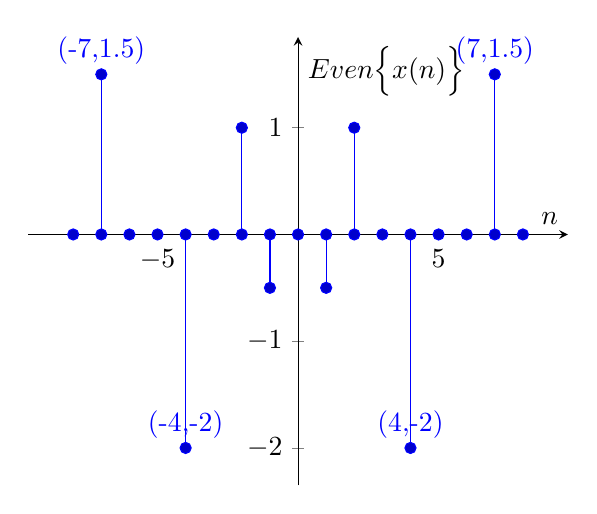
\begin{tikzpicture}
\begin{axis}[axis lines=middle,enlargelimits,
xlabel=$n$,ylabel=$Even\Big\{x(n)\Big\}$,nodes near coords]
\addplot+[point meta=explicit symbolic] coordinates{


(-8,0)

(-7,1.5) [(-7,1.5)]
(-7,0)

(-6,0)

(-5,0)

(-4,0)
(-4,-2)[(-4,-2)]




(-3,0)

(-2,0)
(-2,1)

(-1,0)
(-1,-0.5)

(0, 0)

(1,0)
(1,-0.5)

(2,0)
(2,1)

(3,0)

(4,0)
(4,-2)[(4,-2)]

(5,0)

(6,0)

(7,1.5) [(7,1.5)]
(7,0)

(8,0)
}; 

\end{axis}


\end{tikzpicture}
+
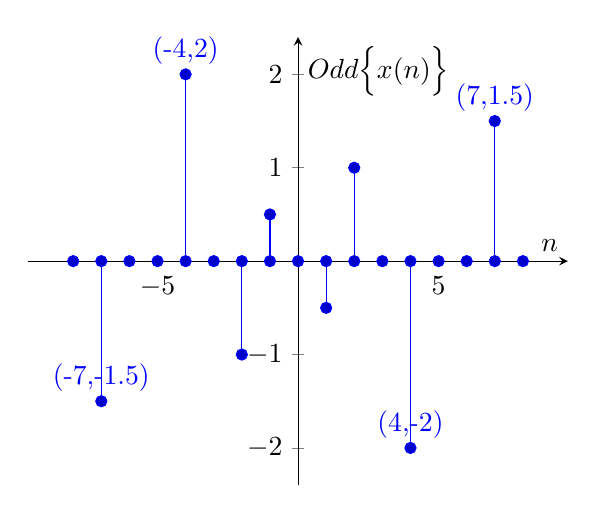
\begin{tikzpicture}
\begin{axis}[axis lines=middle,enlargelimits,
xlabel=$n$,ylabel=$Odd\Big\{x(n)\Big\}$,nodes near coords]
\addplot+[point meta=explicit symbolic] coordinates{


(-8,0)

(-7,-1.5) [(-7,-1.5)]
(-7,0)

(-6,0)

(-5,0)

(-4,0)
(-4,2)[(-4,2)]

(-3,0)

(-2,0)
(-2,-1)

(-1,0)
(-1,0.5)

(0, 0)

(1,0)
(1,-0.5)

(2,0)
(2,1)

(3,0)

(4,0)
(4,-2)[(4,-2)]

(5,0)

(6,0)

(7,1.5) [(7,1.5)]
(7,0)

(8,0)
}; 

\end{axis}


\end{tikzpicture}
.\\\\\\\\
.\hspace{1cm} Even\Big\{x(n)\Big\} = $\frac{1}{2}$[x(n) + x(-n)]\hspace{3.2cm}Odd\Big\{x(n)\Big\}  = $\frac{1}{2}$[x(n) - x(-n)]\\\\\\
As a result, addition of these plots will give us x(n) in Figure 2.
\newpage

\item 
    \begin{enumerate}
    \item %write the solution of q6a 
    y(t) = x(2t-3)\\\\
    $\Rightarrow$ This system has memory, because output signal y(t) depends on the present and past value of the input signal x(t).\\\\
    $\Rightarrow$ A system is stable for an output signal [y(t)] which is bounded for any bounded input signal [x(t)]. For a constant A $>$ 0, $|$x(t)$| <$ A for all t. For a constant B $>$ 0, $|$y(t)$| <$ B for all t. Let x(t) = u(t) [u(t) is a bounded signal]. If y(t) is bounded then system is stable.\\\\
    
    \begin{tikzpicture}[domain=0:2.5] 
    
    \draw[->] (-0.2,0) -- (3,0) node[right] {$t$}; 
    \draw[->] (0,-0.2) -- (0,3) node[above] {$u(t)$};
    \draw[color=red] plot (\x,1); 
    \end{tikzpicture}
    \hspace{2cm} and \hspace{2cm}
    \begin{tikzpicture}[domain=0:4]
    
    \draw[->] (-0.2,0) -- (3,0) node[right] {$t$}; 
    \draw[->] (0,-0.2) -- (0,3) node[above] {$y(t) = u(2t-3)$};
    \draw[color=red] plot (\x/2 + 1,1) ; 
    \draw[color=red] plot (1, \x/4) node[above] {$(3,1)$}; 
    \end{tikzpicture}
    .\\\\\\
    Shifting and scaling the time doesn't effect the value of signal u(t). We just shift the signal 3 times right. Hence, this system is stable.\\\\
    $\Rightarrow$ This system depends on past value of input signal x(t). Also, there is no dependence of future value of x(t). As a result, the system is causal.\\\\
    $\Rightarrow$ Let $x_{1}$(t) $\rightarrow$  System $\rightarrow y_{1}$(t) \hspace{5cm} $x_{2}$(t) $\rightarrow$  System $\rightarrow y_{2}$(t)\\\\
    .\hspace{0.7cm} $y_{1}$(t) = $x_{1}$(2t-3) \hspace{6.7cm} $y_{2}$(t) = $x_{2}$(2t-3)\\\\\\
    $y_{1}$(t) + $y_{2}$(t) = $x_{1}$(2t-3) + $x_{2}$(2t-3)\\\\
    a$x_{1}$(t) + b$x_{2}$(t) = a$x_{1}$(2t-3) + b$x_{2}$(2t-3)\\\\
    So, a$y_{1}$(t) + b$y_{2}$(t) = a$x_{1}$(t) + b$x_{2}$(t)\\\\
    Finally, the system is linear.\\\\\\
    
    $\Rightarrow$ It has an one-to-one mapping. So, the system is invertible. \hspace{2cm} $y^{-1}$ = x ($\frac{t+3}{2}$)\\\\\\
    $\Rightarrow$ Let $x_{1}$(t) $\rightarrow$  System $\rightarrow y_{1}$(t) \hspace{5cm} $x_{2}$(t) $\rightarrow$  System $\rightarrow y_{2}$(t)\\\\
    .\hspace{10.3cm} $x_{2}$(t) = $x_{1}$(t-$t_{0}$)\\\\
    .\hspace{0.7cm} $y_{1}$(t) = $x_{1}$(2t-3) \hspace{6.7cm} $y_{2}$(t) = $x_{1}$(2t-2$t_{0}$-3)\\\\\\
    $y_{1}$(t-$t_{0}$) = $x_{1}$(2t-2$t_{0}$-3). Then, $y_{2}$(t) =  $y_{1}$(t-$t_{0}$). Hence, the system is time-invariant.\\\\
    
    \item %write the solution of q6b
    y(t) = tx(t)\\\\\\
    $\Rightarrow$ The system is memoryless because output signal y(t) doesn't depend on the past value of input signal x(t). For y(t) = h(x(t- $t_{o}$)) $t_{o}$ = 0 for all t\\\\\\
    $\Rightarrow$ Let x(t) = u(t). If y(t) is bounded then the system is stable.\\\\
    \begin{tikzpicture}[domain=0:2.5] 
    
    \draw[->] (-0.2,0) -- (3,0) node[right] {$t$}; 
    \draw[->] (0,-0.2) -- (0,3) node[above] {$u(t)$};
    \draw[color=red] plot (\x,1); 
    \end{tikzpicture}
    \hspace{2cm} and \hspace{2cm}
     \begin{tikzpicture}[domain=0:2.5] 
    
    \draw[->] (-0.2,0) -- (3,0) node[right] {$t$}; 
    \draw[->] (0,-0.2) -- (0,3) node[above] {$t.u(t)$};
    \draw[color=red] plot (\x,\x); 
    \end{tikzpicture}
    .\\\\\\
    Input signal x(t) is bounded; but output signal y(t) is not bounded. Hence, the system is not stable.\\\\\\
    $\Rightarrow$ The system is causal because it is independent of future value of input signal x(t).\\ y(t) = h(x(t- $t_{o}$)) $t_{o}$ = 0 for all t\\\\\\
    $\Rightarrow$ Let $x_{1}$(t) $\rightarrow$  System $\rightarrow y_{1}$(t) \hspace{5cm} $x_{2}$(t) $\rightarrow$  System $\rightarrow y_{2}$(t)\\\\
    .\hspace{0.7cm} $y_{1}$(t) = $t.x_{1}$(t) \hspace{6.7cm} $y_{2}$(t) = $t.x_{2}$(t)\\\\\\
    $y_{1}$(t) + $y_{2}$(t) = t.[$x_{1}$(t) + $x_{2}$(t)]\\\\
    a.$x_{1}$(t) + b.$x_{2}$(t) = a.t$x_{1}$(t) + b.t$x_{2}$(t)\\\\
    So, a.$y_{1}$(t) + b.$y_{2}$(t) = a.$x_{1}$(t) + b.$x_{2}$(t). Finally, the system is linear.\\\\\\
    $\Rightarrow$ It has an one-to-one mapping. So, the system is invertible. \hspace{2cm} $y^{-1}$ = x(t).$\frac{1}{t}$\\\\\\
    $\Rightarrow$ Let $x_{1}$(t) $\rightarrow$  System $\rightarrow y_{1}$(t) \hspace{5cm} $x_{2}$(t) $\rightarrow$  System $\rightarrow y_{2}$(t)\\\\
    .\hspace{10.3cm} $x_{2}$(t) = $x_{1}$(t-$t_{0}$)\\\\
    .\hspace{0.7cm} $y_{1}$(t) = t.$x_{1}$(t) \hspace{6.7cm} $y_{2}$(t) = t.$x_{1}$(t-$t_{0}$)\\\\\\
    $y_{1}$(t-$t_{0}$) = (t-$t_{0}$)$x_{1}$((t-$t_{0}$)). Then, $y_{2}$(t) =  $y_{1}$(t-$t_{0}$). Hence, the system is time-varying.\\\\
    
    \item %write the solution of q6c
    y(n) = x(2n-3)\\\\
    $\Rightarrow$ This system has memory, because output signal y(n) depends on the present and past value of the input signal x(n).\\\\\\
    $\Rightarrow$ Let x(n) = u(n). If y(n) is bounded then the system is stable.\\\\
    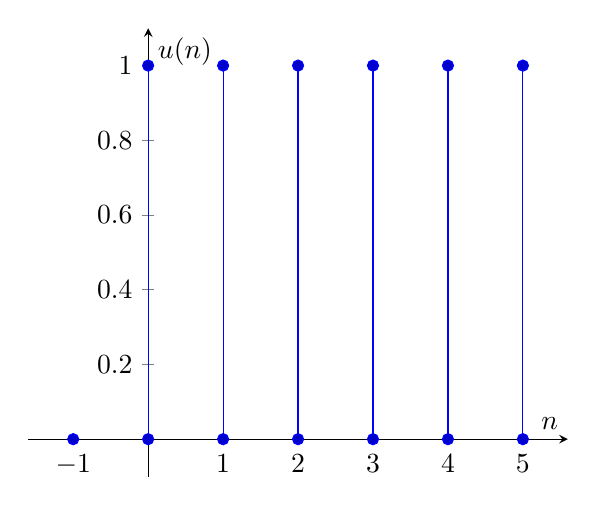
\begin{tikzpicture}
\begin{axis}[axis lines=middle,enlargelimits,
xlabel=$n$,ylabel=$u(n)$]
\addplot+[point meta=explicit symbolic] coordinates{

(-1,0)

(0, 0)
(0,1)

(1,0)
(1,1)

(2,0)
(2,1)

(3,0)
(3,1)

(4,0)
(4,1)

(5,0)
(5,1)

}; 

\end{axis}

\end{tikzpicture}
\hspace{1cm} and \hspace{1cm}
    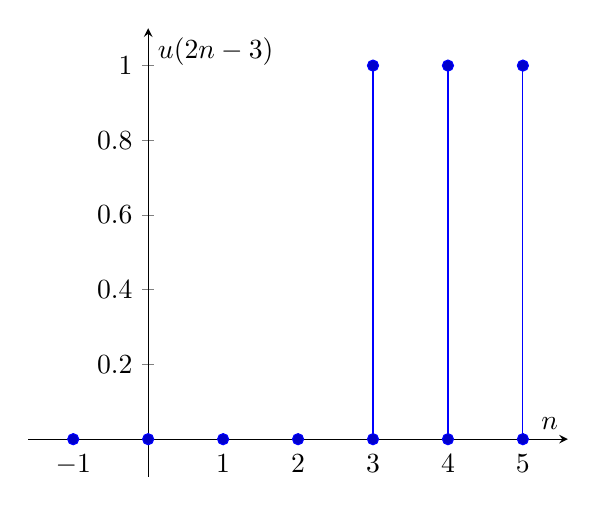
\begin{tikzpicture}
\begin{axis}[axis lines=middle,enlargelimits,
xlabel=$n$,ylabel=$u(2n-3)$]
\addplot+[point meta=explicit symbolic] coordinates{

(-1,0)

(0, 0)

(1,0)

(2,0)

(3,0)
(3,1)

(4,0)
(4,1)

(5,0)
(5,1)
}; 

\end{axis}

\end{tikzpicture}
.\\\\\\\\
    Sifting and scaling doesn't effect the value of signal u(n). We just shifted the signal 3 times right. Then the system is stable.\\\\\\
    $\Rightarrow$ This system depends on future value of input signal x(n). For n = 5  y[5] = x[7]. Hence, the system is not causal.\\\\\\
     $\Rightarrow$ Let $x_{1}$(n) $\rightarrow$  System $\rightarrow y_{1}$(n) \hspace{5cm} $x_{2}$(n) $\rightarrow$  System $\rightarrow y_{2}$(n)\\\\
    .\hspace{0.7cm} $y_{1}$(n) = $x_{1}$(2n-3) \hspace{6.7cm} $y_{2}$(n) = $x_{2}$(2n-3)\\\\\\
    $y_{1}$(n) + $y_{2}$(n) = $x_{1}$(2n-3) + $x_{2}$(2n-3)\\\\
    a.$x_{1}$(n) + b.$x_{2}$(n) = a$x_{1}$(2n-3) + b$x_{2}$(2n-3)\\\\
    So, a.$y_{1}$(n) + b.$y_{2}$(n) = a.$x_{1}$(n) + b.$x_{2}$(n). Finally, the system is linear.\\\\\\
    $\Rightarrow$ $y^{-1}$ = x(.$\frac{n+3}{2}$) is not invertible, because in some values of x(n) the output signal y(n) takes values which is not integer.\\\\\\
    $\Rightarrow$ Let $x_{1}$(n) $\rightarrow$  System $\rightarrow y_{1}$(n) \hspace{5cm} $x_{2}$(n) $\rightarrow$  System $\rightarrow y_{2}$(n)\\\\
    .\hspace{10.3cm} $x_{2}$(n) = $x_{1}$(n-$n_{0}$)\\\\
    .\hspace{0.7cm} $y_{1}$(n) = $x_{1}$(2n-3) \hspace{6.7cm} $y_{2}$(n) = $x_{1}$(2n-2$n_{0}$-3)\\\\\\
    $y_{1}$(n-$n_{0}$) = $x_{1}$(2n-2$n_{0}$-3). Then, $y_{2}$(n) =  $y_{1}$(n-$n_{0}$). Hence, the system is time-varying.\\\\
    
    
    
    
    \item %write the solution of q6d
    y(n) = $\sum_{k=1}^{\infty}$x(n-k)\\\\
    
   $\Rightarrow$ This system has memory, because output signal y(n) depends on the present and past value of the input signal x(n). For y = 0, y[0] = x[-1] + x[-2] ... 0 $>$ -1,-2... \\\\\\
    $\Rightarrow$ For any bounded input x(n) it has unbounded output y(n) so it is not stable.\\\\\\
    $\Rightarrow$ This system depends on past value of input signal x(n). There is no dependence on future value of x(n). For any n  $\rightarrow$ n-k $<$ n in k from zero to infinity. Hence, the system is causal.\\\\\\
   $\Rightarrow$ Let $x_{1}$(n) $\rightarrow$  System $\rightarrow y_{1}$(n) \hspace{5cm} $x_{2}$(n) $\rightarrow$  System $\rightarrow y_{2}$(n)\\\\
    .\hspace{0.5cm} $y_{1}$(n) = $\sum_{k=1}^{\infty} x_{1}$(n-k) \hspace{6cm} $y_{2}$(n) = $\sum_{k=1}^{\infty} x_{2}$(n-k)\\\\\\
    $y_{1}$(n) + $y_{2}$(n) = $\sum_{k=1}^{\infty} x_{1}$(n-k) + $\sum_{k=1}^{\infty} x_{2}$(n-k)\\\\
    a.$x_{1}$(n) + b.$x_{2}$(n) = a$\sum_{k=1}^{\infty} x_{1}$(n-k) + b$\sum_{k=1}^{\infty} x_{2}$(n-k)\\\\
    So, a.$y_{1}$(n) + b.$y_{2}$(n) = a.$x_{1}$(n) + b.$x_{2}$(n). Finally, the system is linear.
    \newpage
   
    $\Rightarrow$ x[n] = y[n+1] - y[n] so it is invertible.\\\\\\
    $\Rightarrow$ Let $x_{1}$(n) $\rightarrow$  System $\rightarrow y_{1}$(n) \hspace{5cm} $x_{2}$(n) $\rightarrow$  System $\rightarrow y_{2}$(n)\\\\
    .\hspace{10.3cm} $x_{2}$(n) = $x_{1}$(n-$n_{0}$)\\\\
    .\hspace{0.7cm} $y_{1}$(n) = $\sum_{k=1}^{\infty} x_{1}$(n-k) \hspace{5.7cm} $y_{2}$(n) = $\sum_{k=1}^{\infty} x_{1}$(n-$n_{0}$-k)\\\\\\
    $y_{1}$(n-$n_{0}$) = $\sum_{k=1}^{\infty} x_{1}$(n-$n_{0}$-k). Then, $y_{2}$(n) =  $y_{1}$(n-$n_{0}$). Hence, the system is time-invariant.\\\\
  
    \end{enumerate}

\end{enumerate}
\end{document}